% Created 2025-02-27 Thu 15:15
% Intended LaTeX compiler: pdflatex
\documentclass[11pt]{article}
\usepackage[utf8]{inputenc}
\usepackage[T1]{fontenc}
\usepackage{graphicx}
\usepackage{longtable}
\usepackage{wrapfig}
\usepackage{rotating}
\usepackage[normalem]{ulem}
\usepackage{amsmath}
\usepackage{amssymb}
\usepackage{capt-of}
\usepackage{hyperref}
\usepackage[danish, ]{babel}
\usepackage[margin=2.5cm]{geometry}
\usepackage{lmodern}
\usepackage[style=verbose-ibid,backend=bibtex]{biblatex}
\addbibresource{bibliography.bib}
\hypersetup{colorlinks, linkcolor=blue, urlcolor=blue}
\author{Alexander Knudsen, Andreas Jensen og Jeppe Bøgeskov}
\date{\today}
\title{Teknologiprojekt -- Fremtidens levevis}
\hypersetup{
 pdfauthor={Alexander Knudsen, Andreas Jensen og Jeppe Bøgeskov},
 pdftitle={Teknologiprojekt -- Fremtidens levevis},
 pdfkeywords={},
 pdfsubject={},
 pdfcreator={Emacs 29.4 (Org mode 9.7.11)}, 
 pdflang={Dk}}
\begin{document}

\newgeometry{top=2.0cm, bottom=2.0cm}
\begin{titlepage}
    \centering

    \vspace*{1cm}

    % Title and subtitle are enclosed between two rules.
    \rule{\textwidth}{1pt}

    % Title
    \vspace{.7\baselineskip}
    {\huge \textbf{Projekt 1 - Krisen kradser}}

    % Subtitle
    \vspace*{.5cm}
    {\LARGE Efterårssemester 2024}

    \rule{\textwidth}{1pt}

    \vspace{1cm}

    % Set this size for the remaining titlepage.
    \large

    % Authors side by side, using two minipages as a trick.

    \begin{table}[h]
        \centering
        \begin{tabular}{cc}
            \begin{minipage}{.5\textwidth}
                \centering
                Jeppe Bøgeskov Bech \\
                {\normalsize \url{jepp9920@zbc.dk}}
            \end{minipage}
            &
            \begin{minipage}{.5\textwidth}
                \centering
                Alexander Schade Knudsen \\
                {\normalsize \url{alex245h@zbc.dk}}
            \end{minipage}
        \end{tabular}

        \vspace{1cm} % Adds vertical space between the rows

        \begin{minipage}{.5\textwidth}
            \centering
            Andreas Jensen \\
            {\normalsize \url{andr328q@zbc.dk}}
        \end{minipage}
    \end{table}








    % More authors can be inserted here with additional minipages.

    \vspace{1cm}

    % Report logo.
    \fbox{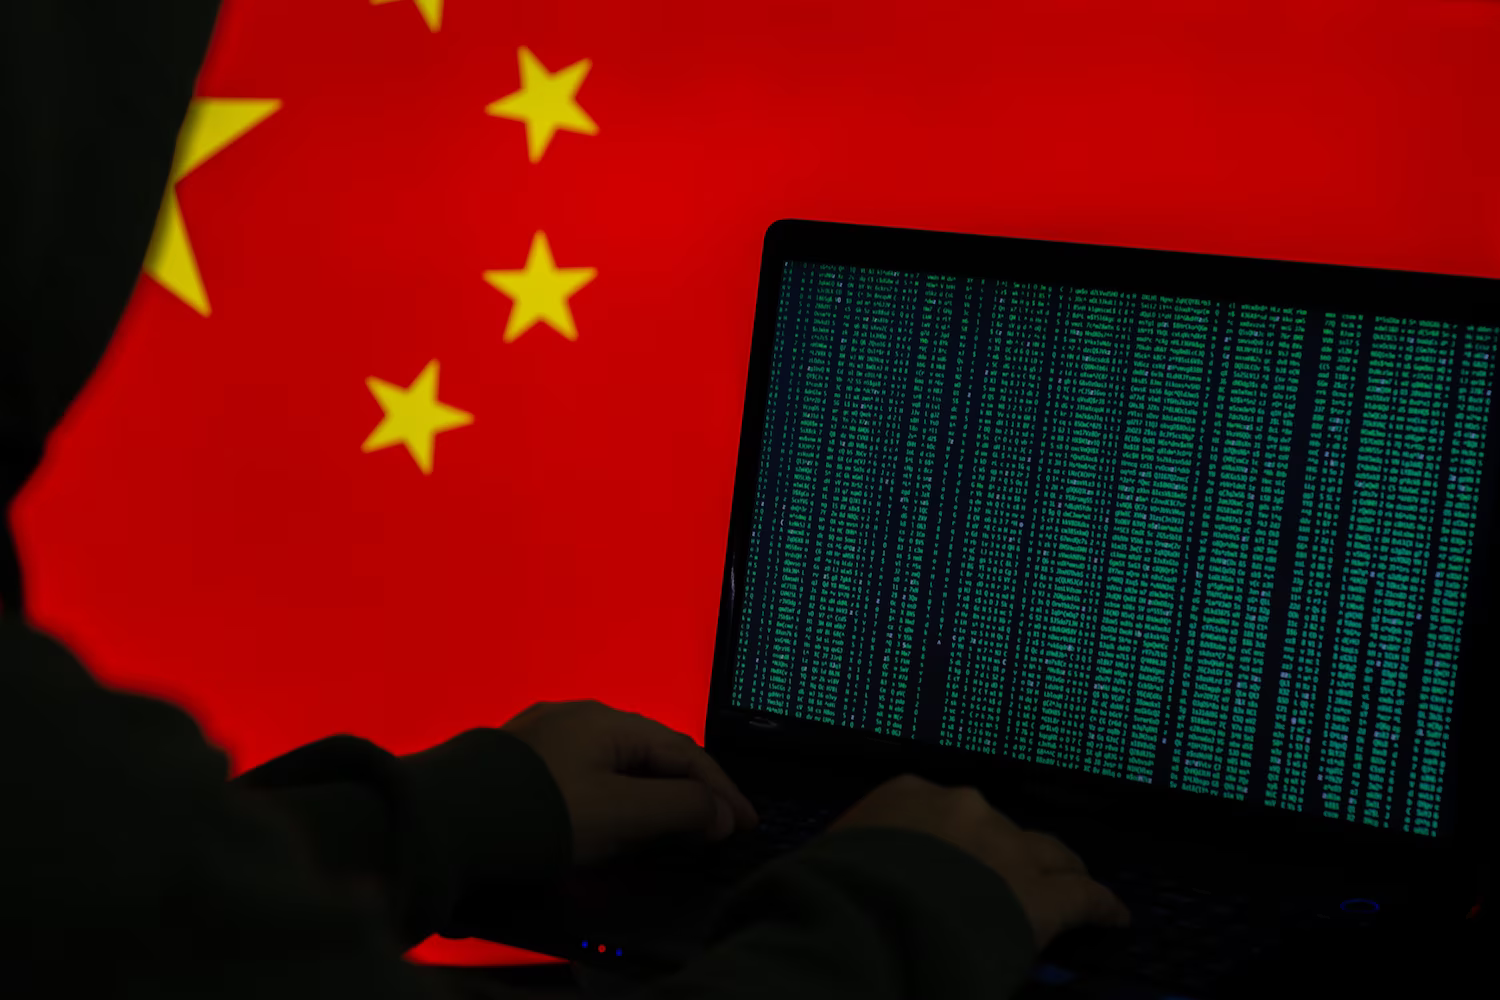
\includegraphics[width=.7\textwidth]{./assets/forsidebillede.png}}

    \vfill

    % University and date information at the bottom of the titlepage.
    2. x \\
    ZBC Handels- og Teknisk gymnasium Slagelse \\
    Akademisk år 2024-2025 \\
    \today
\end{titlepage}


\restoregeometry
\tableofcontents
\newpage
\section{Abstract}
\label{sec:org6419ad8}
In this report, is the work process and descisions leading to creating a smart home system that prioritises data security and self-custody.
\section{Forord}
\label{sec:org4e437e0}
I forbindelse med projektet og produktudvikling vil vi gerne rette en tak til vores faglærer, Henrik Poulsen.
\section{Indledning}
\label{sec:org6d9531c}
\subsection{Projektstyring}
\label{sec:org5e3ff51}
\subsubsection{Oplæg}
\label{sec:orgbec7f1d}
Heri projektet arbejdes der med casen, der omhandler 'bolig'.
\subsubsection{Tidsstyring}
\label{sec:org730faaa}
\begin{itemize}
\item Startdato: 9. december 2024
\item Slutdato: 7. marts 2025
\end{itemize}
\begin{enumerate}
\item Gantt-diagram
\label{sec:orgb1d2daa}
\end{enumerate}
\subsection{Problemidentifikation}
\label{sec:orgfafb1b0}
Indenfor temaet er der en række forskellige emner, som kunne være relevante at arbejde med, herunder high-tech-løsninger. Grundet gruppens kompetencer, er denne valgt, hvorfor problemidentifikation er afgrænset hertil.
\subsubsection{Samfundsmæssige problemstilling}
\label{sec:orga952bf5}
I indledningen af problemidentifikationen fremgik det hurtigt, at nogle af de største smart home løsninger kommer fra udenlandske firmaer, herunder Google, Apple, Amazon, men også firmaer der er blevet kritiseret meget, såsom TP-Link. (indsæt tplink-kilde)

Desuden beskrives i sikkerhedsblad også, hvordan samtlige IoT-enheder har været anvendt af kinesiske, statssponsorede, hackere til i botnet (indsæt forklaring omkring botnet) til at angribe kritiske sektorer i det amerikanske samfund, såsom militær-, udannelseinstitutioner og telekommunikationsløsninger. (indsæt securityweek-kilde)

Ifl. Forsvarets Efterretningstjeneste, vurderer Center for Cybersikkerhed, at Ruslands øgede risikovillighed i forhold til at bruge hybride virkemidler mod NATO-lande, herunder Danmark, også omfatter destruktive cyberangreb. (indsæt \url{https://www.fe-ddis.dk/da/arbejdsomrade-a/den-hybride-trussel/} kilde) Indtil videre er der ikke anmeldt angreb via IoT ting, men det kan ikke udelukkes, at Rusland, som er allieret med Kina, potentielset ville kunne udnytte Kinesiske firmaers adgang til data iagt af deres markedsandel indenfor IoT-things.

Grundet, at det Kommunistiske Kinesiske Parti har regeringsmagten i Kina, medfører dette totalitær lovgivning, der nemlig gør, at partiet kan indkræve samtlige data fra firmaer, der oppererer til lands (indsæt kilde). Potentialet i dette alene, er nok til at refærdiggøre udvikling af et alternativt produkt, såsom det, der heri rapporten beskrives.

Således er der få alternativer til status quo, som der herfra kan viderudvikles på. Se afsnit om idegenerering (\ref{sec:org12d3e0c}).
\subsection{Idegenerering}
\label{sec:org12d3e0c}
Alternativerne til status quo-IoT-løsningerne er følgende:
\begin{itemize}
\item Afdigitalisering af nuværende løsninger
\item Udvikling af decentraliserede løsninger, der involverer self-custody (indsæt fodnote)
\item Udvikling af centraliseret løsninger, udgivet af et troværdigt firma i et land, der ikke kræver udleveringen af data fra sine brugere
\end{itemize}
\subsection{Idesortering (lyskurvemetoden)}
\label{sec:orgb65406b}
Den første løsning indebærer, at man bevæger sig væk fra vores oprindelige afgrænsning af fokusområde, nemlig det digitale, hvilket i øvrigt findes i forvejen, hvorfor markedet for dette vurderes mættet.

Desuden grundet gruppens IT-kompetencer, virker de to resterende løsninger som mere kompatible med gruppen. Imellem disse to ideer, vurderes det, at den mere spændende løsning er at lave det decentraliseret med en såkaldt FOSS-løsning, se kapitlet herom (indsæt kapitellink)
\subsection{Afgrænsning}
\label{sec:orgc46d8ef}
Da en total smarthjemsløsning er meget omfattende, vælges der herfor at fokusere på enkelte dele af en sådan løsning. I dette tilfælde er det endelige produkt et proof-of-concept, hvori en smarthub kan sende signaler og modtage signaler til andre eheder på et lokalt netværk. Desuden skal denne kunne fjernbetjenes igennem en styringsapplikation.
\subsection{Problemformulering}
\label{sec:orgef4d52f}
\section{Problemanalyse}
\label{sec:org3679584}

I problemanalysen er problemstillingen blevet yderligere konkretiseret bl.a. ved et problemtræ (indsæt link til problemtræ)
\begin{figure}[htbp]
\centering
\includegraphics[width=.9\linewidth]{assets/Problemtræ.png}
\caption{Viser projektets problemtræ}
\end{figure}
\subsection{Interessentanalyse}
\label{sec:org976cef3}
\subsubsection{Ekstern interessenter}
\label{sec:orgf2dab0a}
\begin{itemize}
\item NGO'er
\end{itemize}
\subsubsection{Gidsel}
\label{sec:org34c7521}
\begin{itemize}
\item Konsumenter
\end{itemize}
\subsubsection{Grå eminence}
\label{sec:orgaa235ac}
\begin{itemize}
\item Konkurrenter
\end{itemize}
\subsubsection{Ressourceperson}
\label{sec:org63a3f15}
\begin{itemize}
\item Staten
\end{itemize}
\subsection{HV-modellen}
\label{sec:org6b97fc3}
\subsubsection{Hvad}
\label{sec:orgbaa59e1}
\begin{enumerate}
\item Et konkurrencealternativ
\end{enumerate}
\subsubsection{Hvorfor}
\label{sec:orgda4cb7c}
\begin{enumerate}
\item For at få markedsandel på vestlige hænder
\end{enumerate}
\subsubsection{Hvem}
\label{sec:org4e76554}
\begin{enumerate}
\item Et privat firma.
\item Kinesiske firmaer påvirkes, her negativt.
\end{enumerate}
\subsubsection{Hvor}
\label{sec:org442bab2}
\begin{enumerate}
\item Resten af vestlige lande.
\end{enumerate}
\subsubsection{Hvordan}
\label{sec:org66417d5}
\begin{enumerate}
\item Decentralt IoT-system
\end{enumerate}
\section{Produktprincip}
\label{sec:orga77d6f9}
\subsection{Konkurrentanalyse}
\subsubsection{IKEA}
IKEA leverer IoT-produkter, som f.eks. smarte lamper, stik samt smart-rullegardiner. Fordelen ved IKEAs produkter er, at de er relativt billige sammenlignet med andre produkter på markedet, at de indgår i et veludviklet og etableret smart-økosystem samt at de er lette at installere.
IKEAs produkter bliver fremstillet af tvangsarbejdere af bla. hviderussiske fanger. \footfullcite{IKEA} grudnet geopolitiske omstændigheder kan det være problematisk at produkterne bliver fremstillet i Hviderusland.\Ref{sec:orga952bf5}
\begin{figure}[htbp]
\centering
\fbox{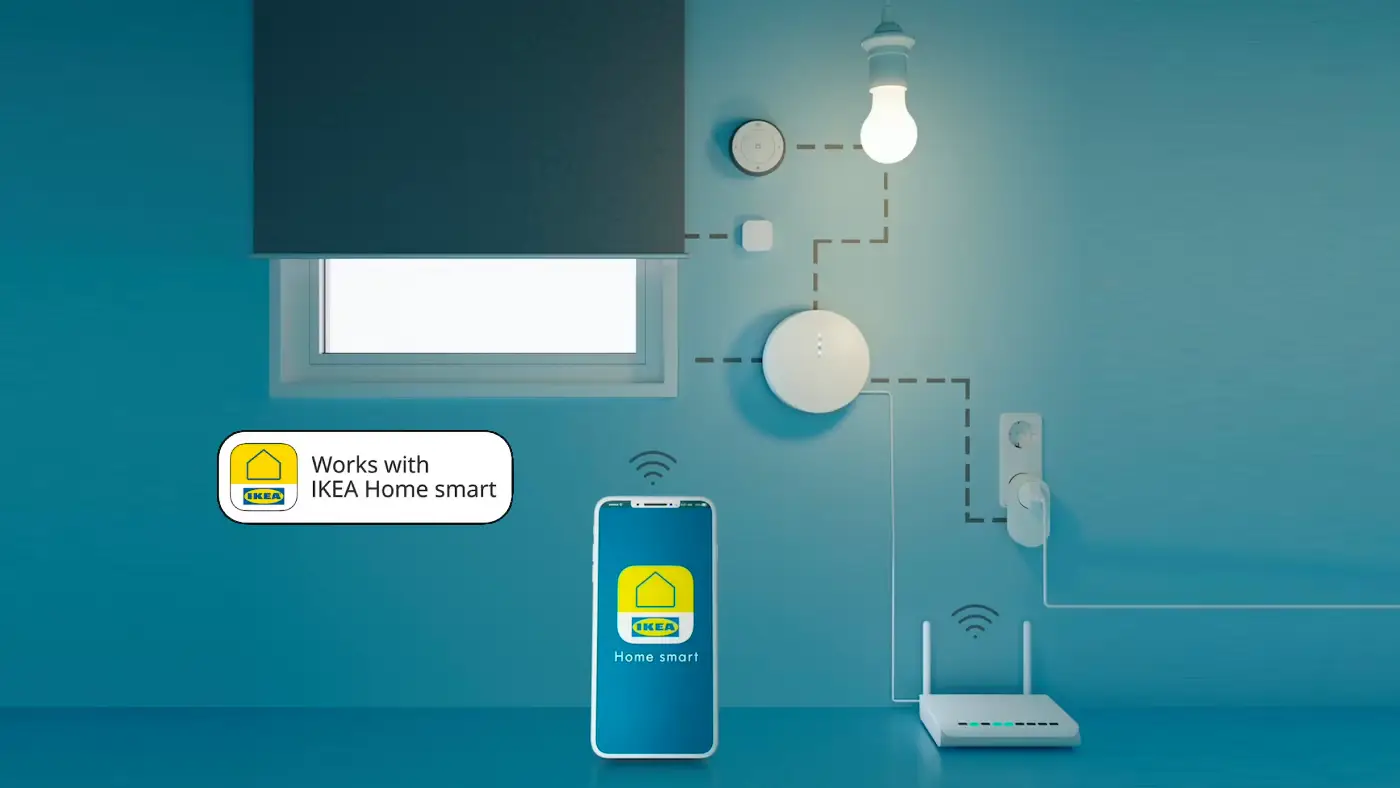
\includegraphics[width=.75\linewidth]{assets/Ikea-smart-home.png}}
\caption{Viser en illustration af IKEA smart-home}
\end{figure}
\subsubsection{TP-Link}
Problematikkerne vedrørende TP-Link er tideligere blevet beskrevet i afsnit \ref{sec:orga952bf5}.
\subsubsection{Xiaomi}
Xiaomi er et kinesisk firma, der leverer en lang række smart-hjemme-produkter med et meget stort udvalg. Fordelene ved Xiaomi er, at brugeren kan købe alle smart-hjem-produkterne under ét firma, hvilket gør det lettere at kontrollere, da de bruger en samlet platform til at styre alle deres produkter. Ulempen ved Xiaomi er, at det er et Kinesisk firma, hvilket udgør en stor risiko\ref{sec:orga952bf5}. Produkterne fra Xiaomi er også relativt billige sammenlignet med andre mere premium produkter på markedet.

\begin{figure}[htbp]
\centering
\fbox{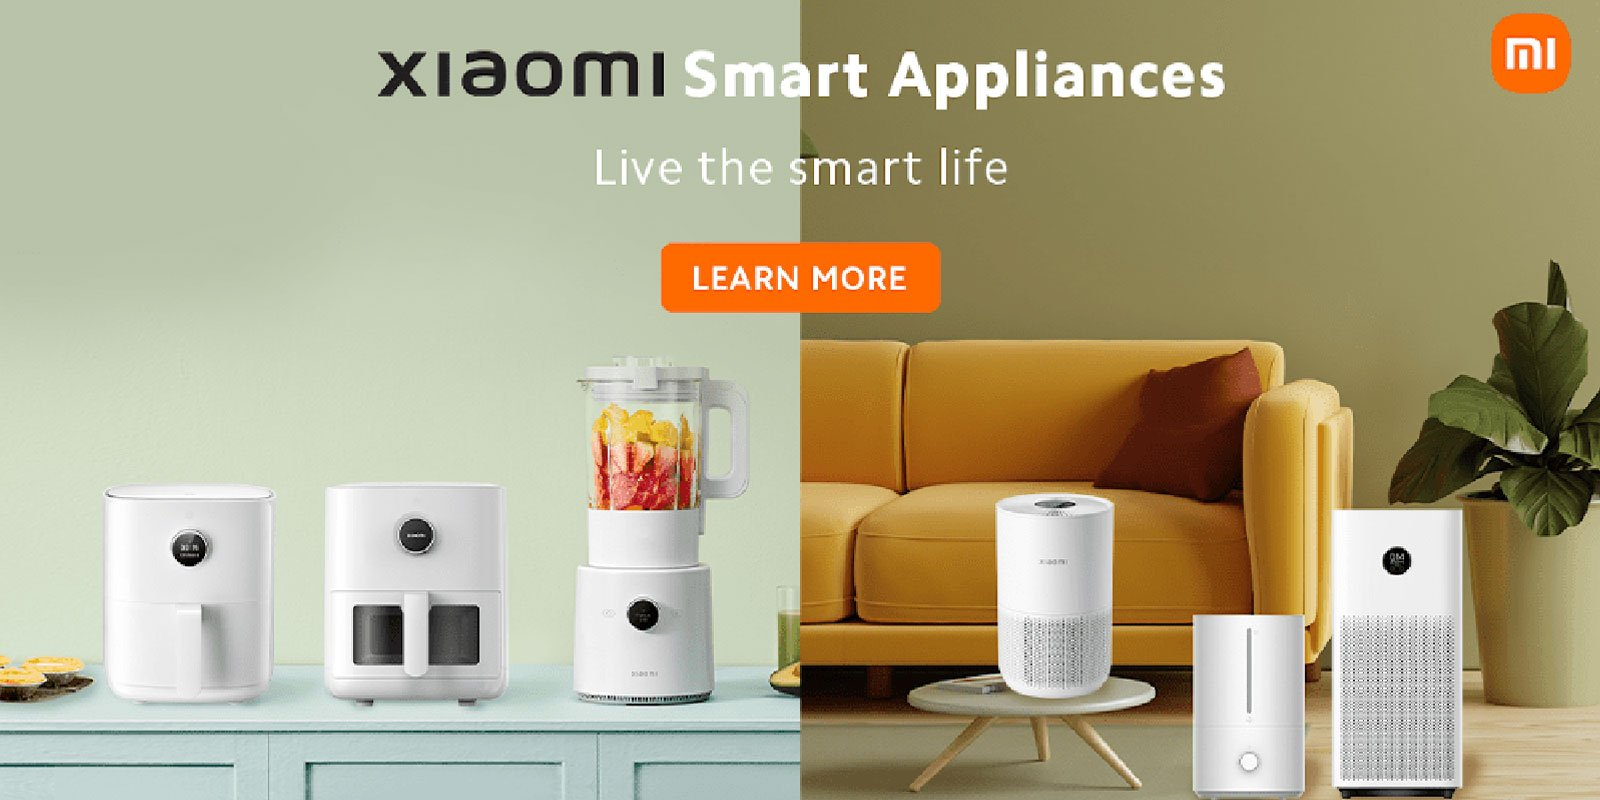
\includegraphics[width=.75\linewidth]{assets/xiaomi.jpg}}
\caption{Viser en illustration af Xiaomi smart-home}
\end{figure}

\subsubsection{Huawei}
Huawei er også en kinesisk virksomhed, som udbyder en række smart-produkter. Den amerikanske start har valgt at banlyse salg og import af nye huawei-produkter. Dette gjorde man fordi man frygtede at der var en risiko for såkaldte "bagdøre" (backdoors) i virksomhedens produkter.\footfullcite{huawei}


\section{Produktudformning}
\label{sec:org563ee9e}
\subsection{Software}
\label{sec:org6da2577}
\subsection{Hardware}
\label{sec:orgdbd4fd8}
\section{Produktionsforberedelse}
\label{sec:orge880538}
\subsection{Masseproduktion}
\label{sec:orge66eada}
\section{{\bfseries\sffamily TODO} Realisering}
\label{sec:orgd4c9e64}
\section{{\bfseries\sffamily TODO} Evaluering}
\label{sec:org4ddb451}
\section{{\bfseries\sffamily TODO} Miljøvurdering}
\label{sec:org9bb106c}
\subsection{Hardwarepåvirkning}
\label{sec:org9e89a3f}
\subsection{Softwarepåvirkning (serverpåvirkning)}
\label{sec:org15c2cb6}
\section{Konklusion}
\label{sec:org7454aed}
\end{document}
